% Created 2014-05-12 Mon 11:58
\documentclass[a4,onecolumn,portrait]{article}
\usepackage[utf8]{inputenc}
\usepackage[T1]{fontenc}
\usepackage{fixltx2e}
\usepackage{graphicx}
\usepackage{longtable}
\usepackage{float}
\usepackage{wrapfig}
\usepackage[normalem]{ulem}
\usepackage{textcomp}
\usepackage{marvosym}
\usepackage{wasysym}
\usepackage{latexsym}
\usepackage{amssymb}
\usepackage{amstext}
\usepackage{hyperref}
\tolerance=1000
\usepackage[english]{babel}
\usepackage{ucs}
\usepackage{inputenc}
\usepackage{fontenc}
\usepackage{hyperref}
\usepackage{graphicx}
\usepackage{parskip}
\usepackage{makeidx}
\makeindex
\usepackage{lmodern}
\usepackage{fullpage}
\usepackage{wrapfig}
\usepackage{verbatim}
\usepackage[hang,small]{caption}
\usepackage{float}
\usepackage{fancyhdr}
\setlength{\headheight}{18pt}
\pagestyle{fancyplain}
\author{by Jaromil @ dyne.org}
\date{May 2014}
\title{Jaro Mail 2.0}
\hypersetup{
  pdfkeywords={},
  pdfsubject={},
  pdfcreator={Emacs 24.3.1 (Org mode 8.0.6)}}
\begin{document}

\maketitle
\tableofcontents

\fancyhf{}
\fancyhead[L]{\rule[-2ex]{0pt}{2ex}\small JaroMail manual}
\fancyhead[R]{\rule[-2ex]{0pt}{2ex}\small version 2.0}
\fancyfoot[C]{-- \thepage\ --}
\fancyfoot[R]{\small Dyne.org Foundation}
\fancyfoot[L]{\small Free Software Manual}

\renewcommand{\headrulewidth}{0.4pt}
\renewcommand{\footrulewidth}{0.4pt}

\pagebreak


\section{Introduction}
\label{sec-1}

Jaro Mail is an integrated suite of interoperable tools to manage
e-mail communication in a private and efficient way, without relying
too much on on-line services, in fact encouraging users to store their
email locally.

Rather than reinventing the wheel, this suite reuses existing free and
open source tools and protocols and is mainly targeted for
GNU/Linux/BSD desktop usage.

This manual illustrates the usage of Jaro Mail. The newest version of
this manual is made available on \url{http://files.dyne.org/jaromail/jaromail-manual.pdf}

\subsection{Features}
\label{sec-1-1}

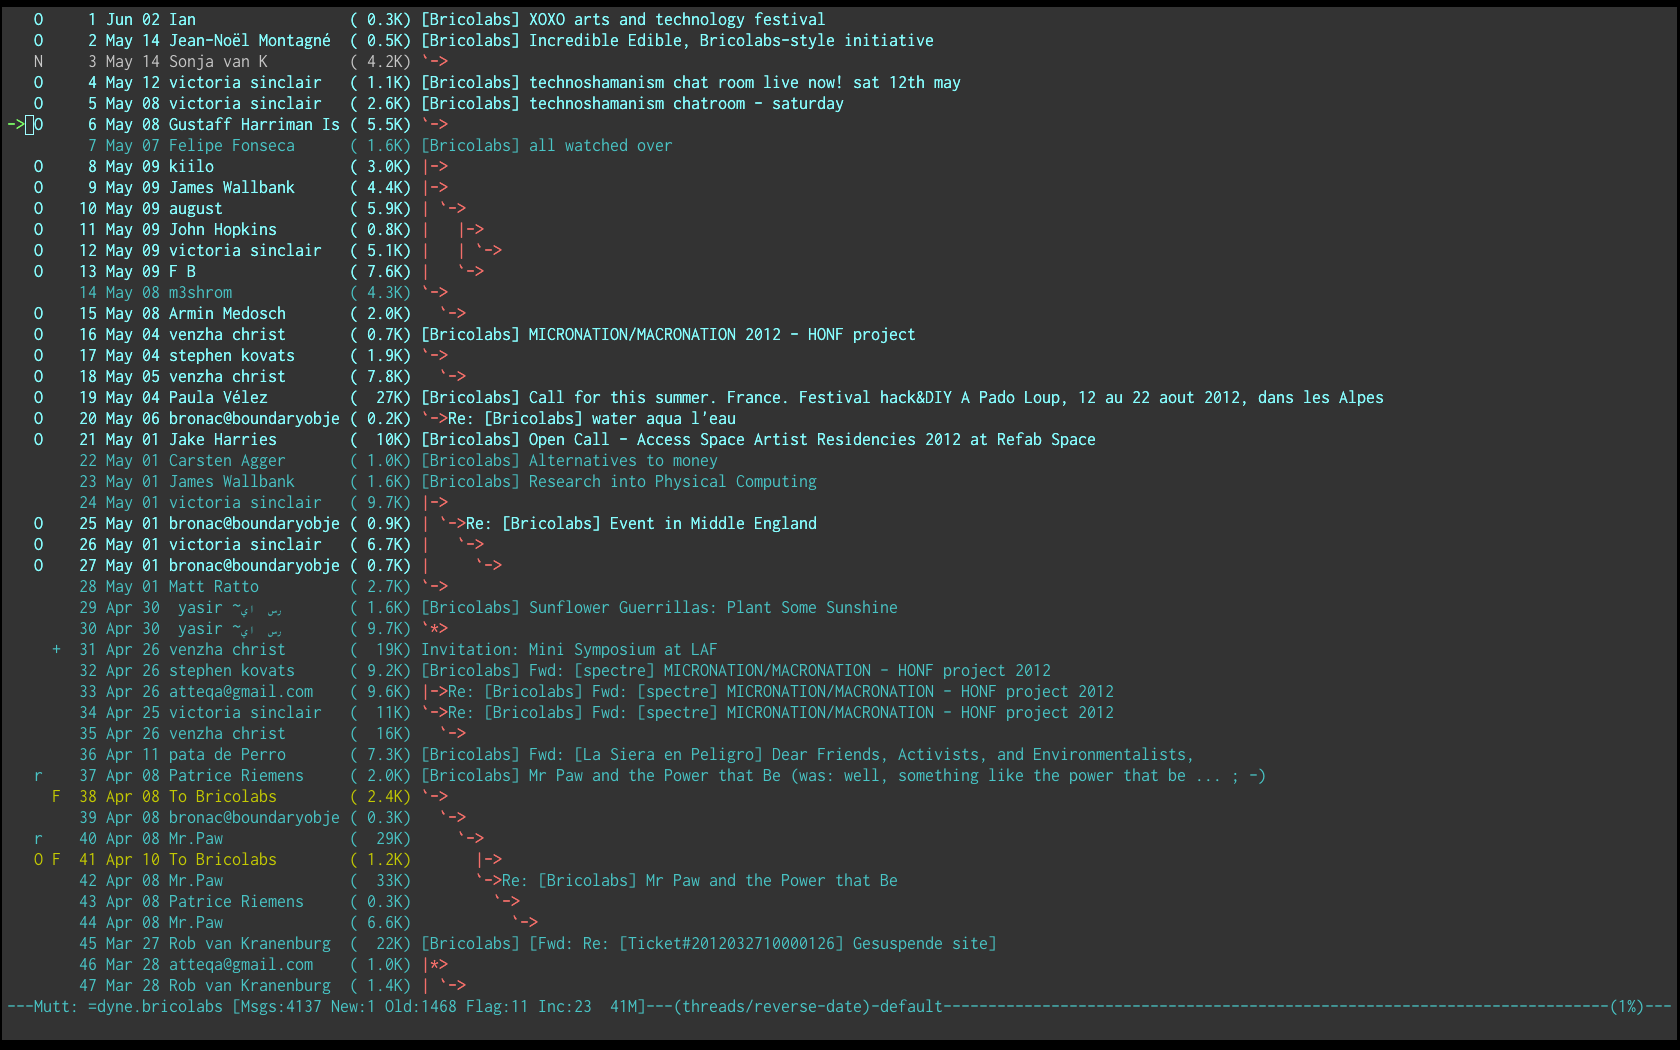
\includegraphics[width=.9\linewidth]{jaromail-shot.jpg}

\footnotesize
\begin{itemize}
\item Minimalistic and efficient interface with message threading
\item Targets intensive usage of e-mails and mailinglists
\item Stores e-mails locally in a reliable format (maildir)
\item Integrates whitelisting and blacklisting, local and remote
\item Can do search and backup by advanced expressions
\item Automatically generates filter rules (procmail, sieve)
\item Imports and exports VCard contacts to its addressbook
\item Computes and shows statistics on mail traffic
\item Encrypts password storage (using keyrings)
\item Provides advanced maildir management tools (rmdupes, backup)
\item Defers connections for off-line operations
\item Checks SSL certificates over (imap, smtp)
\item Supports strong encryption messaging (GnuPG)
\item Multi platform: GNU/Linux/BSD, Apple/OSX
\item Old school, used by its author for the past 10 years
\end{itemize}
\normalsize
\subsection{Vision}
\label{sec-1-2}

\begin{wrapfigure}{r}{0.5\textwidth}
  \begin{center}
    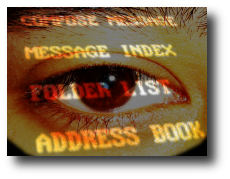
\includegraphics[width=0.48\textwidth]{foster_privacy.png}
  \end{center}
\end{wrapfigure}
The internet offers plenty of free services, on the wave of the Web2.0
fuzz and the community boom, while all private informations are hosted
on servers owned by global corporations and monopolies.

It is important to keep in mind that no-one else better than you can
ensure the privacy of your personal data. Server hosted services and
web integrated technologies gather all data into huge information
pools that are made available to established economical and cultural
regimes.

The vision behind this software is that of sharing a simple and
consistent way to operate e-mail communication with tools that are
available on most platforms and can be as well used remotely over a
secure shell connection.

Jaro Mail aims to facilitate the task of downloading and storing e-mail
archives off-line in a way that they can be still accessible in more
than 10 years time and independently of any software. Nowadays many
users have the habit of keeping all their e-mails on servers,
accessing them through an often clumsy web interface, while
downloading them can free space and improve their privacy.

\pagebreak
\section{Diagram}
\label{sec-2}

A little diagram that clarifies a bit where do we place the components
and actions involved in managing one's email communication:

\begin{figure}
  \begin{center}
    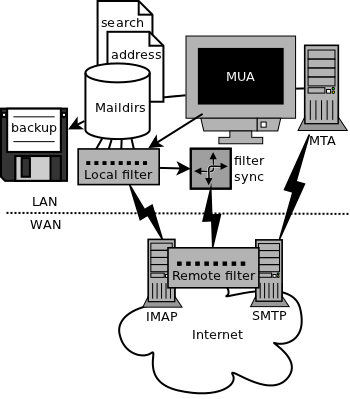
\includegraphics[width=0.4\textwidth]{jaromail-diagram.png}
  \end{center}
\end{figure}
\begin{center}
\begin{tabular}{lll}
Acronym & Function & Software\\
\hline
MUA & Mail User Agent & \href{http://www.mutt.org}{Mutt}\\
MTA & Mail Transport Agent & \href{http://www.fetchmail.info}{Fetchmail}\\
LDA & Local Delivery Agent & Jaro Mail\\
MDA & Remote Delivery Agent & \href{http://en.wikipedia.org/wiki/Sieve_(mail_filtering_language)}{Sieve}\\
SMTP & Mail Delivery Agent & \href{http://msmtp.sourceforge.net}{MSmtp}\\
 & Search engine & \href{http://www.rpcurnow.force9.co.uk/mairix/}{Mairix}\\
 & Addressbook & \href{http://abook.sf.net}{ABook}\\
GPG & Cryptographic Agent & \href{http://www.gnupg.org}{GnuPG}\\
\end{tabular}
\end{center}

\pagebreak
\section{Setup}
\label{sec-3}

\subsection{Build}
\label{sec-3-1}

Jaro Mail needs to be built on GNU/Linux systems.

For Apple/OSX users it comes in a pre-compiled bundle.

\subsubsection{GNU/Linux}
\label{sec-3-1-1}

Some dependencies are needed in order to build this software. The Makefile for GNU/Linux configures the build environment automatically on Debian and Fedora systems, using their packaging to install all needed packages.

The dependencies to be installed on the system for JaroMail are
\begin{itemize}
\item to \textbf{build}: bison flex make autoconf automake sqlite3 libgnome-keyring-dev
\item to \textbf{run}: procmail fetchmail msmtp mutt mairix pinentry abook wipe

To install all needed components (done automatically, requires root):
\end{itemize}

\begin{verbatim}
make
\end{verbatim}

Once compiled then \textbf{make install} will put all JaroMail files in \textbf{/usr/local/share/jaromail}.
\subsubsection{Apple/OSX}
\label{sec-3-1-2}

Apple/OSX users that have no experience in building software can obtain a pre-built universal binary from our download zone on \url{http://files.dyne.org/jaromail/binary}

One can simply drag JaroMail into Applications. When started JaroMail opens a Terminal window preconfigured with its environment, to activate it for any terminal add this to `\textasciitilde{}/.profile`:
\begin{verbatim}
export PATH=/Applications/JaroMail.app/Contents/Resources/jaro/bin:$PATH
\end{verbatim}
\subsection{Install}
\label{sec-3-2}

Installing Jaro Mail once all dependencies are build is fairly
easy: make a directory where all the emails and settings needs to be, change to the directory and init the environment:

\begin{verbatim}
$ mkdir $HOME/Mail
$ cd $HOME/Mail
$ jaro init
\end{verbatim}

Every installation of Jaro Mail is fully reentrant, meaning the directory where it gets initialised contains all maildirs, configurations, filters, whitelist, addressbooks and other necessary files.

A single user can have multiple Jaro Mail installations to permit the complete separation of E-Mail identities.

If called from outside the installation directory, the \textbf{jaro} command will use the environmental variable \textbf{\$JAROMAILDIR} to find out the active installation being in use. If one is using a different installation path then should first change that, i.e:

\begin{verbatim}
export JAROMAILDIR=$HOME/OtherIdentities/Luther/Mail
\end{verbatim}
\section{Configuration}
\label{sec-4}

The place where Jaro Mail is installed (\textbf{\$HOME/Mail} by default)
contains all configuration files.

For Apple/OSX users, this directory is inside their \textbf{\$HOME/Library}, then \textbf{Application Support} and then \textbf{JaroMail}.

From now own, we will call this place the \textbf{Mail directory}.

Inside the \textbf{Mail directory} are all needed configurations to operate JaroMail. Such configurations are in readable plain text files that can be edited using any editor. Inside them there are comments to explain the settings: all comment lines start by '\#' and will be ignored by JaroMail.

The most important files to start configuring are:

\begin{itemize}
\item Identity.txt : set up the way your email identity appear to others
\item Accounts/default.txt : main account configuration (there can be more)
\item Aliases.txt : more email addresses one may receive on the configured accounts
\item Filters.txt : Full set of mailinglist sorting rules
\item Applications.txt : mime type associations to programs used to open attachments
\end{itemize}

\subsection{Send and receive mail}
\label{sec-4-1}

Inside the Mail directory is found the folder \textbf{Accounts} with brief
instructions and default templates to fill with Imap and Smtp account
configurations to fetch mail. A default template will be found in
fresh installations: \textbf{Accounts/default.txt}. The configuration can
be edited with one's favourite text editor, the format of the file
is pretty self-explanatory.

It is possible to have more than one account (simply as a new file
in the Accounts/ directory) and in fact when retreiving e-mails
using the \textbf{jaro fetch} command all accounts will be processed,
unless one is explicitly selected using the \textbf{-a} commandline
option.

The file \textbf{Identity.txt} is also found in the Mail directory and it
contains basic settings on the published user identity (From:
field) and any other Mutt specific configuration directives, such
as custom headers appearing in composed e-mails and the default
GPG\footnote{GPG stands for GNU Privacy Guard, a system to securely
encrypt and decrypt messages and files so that noone can read their
content, even when intercepting the communication.} key to be used when signing and encrypting them.  For
more information about the vast amount of configurations that are
supported please refer to the Mutt documentation\footnote{The Mutt configuration manual is found on \url{http://www.mutt.org/doc/manual} or simply typing 'man mutt' in a console terminal.}
\subsection{Filter mail}
\label{sec-4-2}

In the mail directory a file named \textbf{Filters.txt} can be created and
filled in with rules referencing the contents of the \textbf{From:}
or \textbf{To:} fields of each e-mail that is fetched. The mails matching
will be then saved in the indicated maildirs (created if not
existing) to keep a bit of order, especially useful for mailinglist
users.

The format of the filters configurarion is pretty easy and self
explanatory, an example is found in the appendix of this manual.

\section{Organization}
\label{sec-5}

One of the main goals for Jaro Mail is to organize the e-mail workflow
so that one's attention is dedicated to important communications,
rather than being constantly distracted by various degrees of spam and
the need to weed it out of the mailbox. This ambitious task is pursued
by realizing an integrated approach consisting of flexible
whitelisting and the distinction between mails from known people and
the rest.

\subsection{Folders}
\label{sec-5-1}

First lets start with a categorization of the standard maildirs and a
brief description for each. This information is \textbf{very important} to
understand how Jaro Mail works: these maildirs are standard in Jaro
Mail, here they are listed in order of priority

\begin{center}
\begin{tabular}{ll}
Folder & What goes in there\\
\hline
\textbf{known} & Mails whose sender is known (Whitelist)\\
\textbf{priv} & Unknown sender, we are the explicit destination\\
\textbf{unsorted} & Unknown sender, we are in cc: or somehow reached\\
\textbf{unsorted.ml} & From a mailinglist that we haven't filtered yet\\
\textbf{zz.blacklist} & Mails whose sender is not desired (Blacklist)\\
\end{tabular}
\end{center}

The advantage using such a folder organization is that every time we
open up the mail reader we will be presented with something we are
likely to be most interested in (known people replying our mails) and
progressively, as we will have the time to scroll through, mails from
"new people" or mass mailings of sort. Please note this organization
does not includes spam, which is supposedly weeded out on the server
via spamlists: White/Blacklisting has more to do with our own
selection of content sources than with the generic protection from
random pieces of information.
\subsection{Whitelist}
\label{sec-5-2}

The way whitelisting works if quite crucial to this setup and, at the
same time, is fairly simple since it does not include any automatic
detection, learning filters, Markov chains or Bayesian A/I. We believe
the user should be in full control of prioritizing communication
channels and at the same time constantly able to tweak the setup in an
easy way.

To whitelist an address is sufficient to send it an e-mail: at the
moment the message is sent Jaro Mail will remember the destination
address and prioritize all messages coming back from it.
This we call implicit whitelisting.

To explicitly whitelist an address from inside the mail reader index
press [ \textbf{a} ] while selecting an email, this will add in the whitelist
the sender address (From: header). If you want to add all addresses
reached by the mail (From: To: and Cc: fields) use the same letter
capitalized pressing shift [ \textbf{A} ].

All addresses selected this way will have the privilege of ending up
in your \textbf{known/} folder, plus their name and e-mail will be completed
automatically when composing a new email, pressing the \textbf{Tab} key while
indicating them among the recipients.
\subsection{Blacklist}
\label{sec-5-3}

To blacklist an address instead one can use the [ \textbf{z} ] key while an
e-mail is selected on the index: the sender indicated in the From:
field will be downgraded to the very bottom of your priorities, closes
to spam than the rest, the most infamous \textbf{zz.blacklist/} folder.

To remove addresses from the blacklist, use \textbf{jaro abook blacklist} which will open the addressbook editor where you can delete, add and modify entries.
\subsection{Addressbook}
\label{sec-5-4}

What we call addressbook here basically consists of both the whitelist
and the blacklist. We store both lists in a unique database file in
the Mail dir called *Addressbook*\footnote{Jaro Mail uses sqlite3 as its own database storage}.  In future we may add
similar support for other addressbook formats that people use (GnuPG
keyring, Evolution etc.)\footnote{On Apple/OSX systems Jaro Mail has access to the Mail.app addressbook, so all contacts known in your Mac will be automatically whitelisted}


Both the white and blacklist can be edited using a text interface,
this way you can delete entries for instance (removing them from the
whitelist or blacklist), or add entries by hand (for instance manually
from visit cards), as well you can change details directly (name and
email). To edit the addressbook in Jaro Mail the \textbf{abook} command is
available

\begin{verbatim}
jaro abook
\end{verbatim}

This will open the current whitelist for edit, but one can append
"blacklist" to this commandline to open that one instead.

To quickly dump to the console all names and addresses in the Jaro
Mail addressbook, one can use the \textbf{list} command

\begin{verbatim}
$ jaro list
\end{verbatim}

To search a string across the addressbook, simply use the command
search followed by a string, for instance:

\begin{verbatim}
$ jaro search autistici
\end{verbatim}

will list all addresses @autistici in your addressbook.

Even more useful to interface with other addressbook
software and mobile phones, you can use the \textbf{export} and \textbf{import}
functions to transport your addressbook formatted as a series of
VCards\footnote{A file format standard for electronic business cards, see: \url{http://en.wikipedia.org/wiki/VCard}}.

\begin{verbatim}
$ jaro export
\end{verbatim}

Will create or update the file in \textbf{Mail/jaro/addressbook.vcf}. On the
other hand, the import command will include all entries found in a
given VCard file that have at least one email address.

\begin{verbatim}
$ jaro import 00001.vcf
\end{verbatim}

Imports into the whitelist all contacts found in the 00001.vcf file.
The VCard format is fully compatible with import and export of
contacts in Android mobile phones.

Apple Mac/OSX users can simply run the import command without any arguments

\begin{verbatim}
$ jaro import
\end{verbatim}

Imports all the contacts found in the system addressbook used by Mail.app,
hence making them whitelisted.
\subsection{Organization In Brief}
\label{sec-5-5}

Below a recapitulation of keys related to the white and blacklisting
functionality, to be used in the e-mail index or when an e-mail is
open inside the mail user agent:

\begin{center}
\begin{tabular}{llll}
List & Key & Function & Fields\\
\hline
White & \textbf{a} & Add the sender address & From:\\
White & \textbf{A} (shift) & Add all addresses & From: To: Cc:\\
Black & \textbf{z} & Blacklist the sender & From:\\
\end{tabular}
\end{center}

And here the addressbook commands that are available from the
commandline:

\begin{center}
\begin{tabular}{ll}
Command & Function\\
\hline
\textbf{abook} & edit the addressbook\\
\textbf{list} & list the addressbook\\
\textbf{search} & search a name or address\\
\textbf{export} & export to a VCard file\\
\textbf{import} & import from a VCard file\\
\end{tabular}
\end{center}
\section{Workflow}
\label{sec-6}

This section goes through a scenario of simple usage for Jaro Mail

\subsection{Fetch and read your mail at home}
\label{sec-6-1}

As you acces your computer where Jaro Mail has been configured, you
can open a Terminal and type:

\begin{verbatim}
$ jaro fetch
\end{verbatim}

This will download all new mails.

If you have configured \textbf{fetchall} among the imap account options, then
will delete them from the server, freeing online space.

If you have configured the \textbf{keep} option, which is the default, Jaro
Mail will only download the email that you have not yet read and in
any case it won't delete anything from the server.

\begin{verbatim}
$ jaro
\end{verbatim}

This will open the first folder containing unread emails, starting from
the \textbf{known} folder, then \textbf{priv}, then all the rest.

From there on, pressing \textbf{=} or \textbf{c} you can change the folder and
explore your \textbf{priv} folder, the mailinglist ones as configured by your
Filters.txt, as well your \textbf{unsorted} mails.
\subsection{Write a new mail}
\label{sec-6-2}

If you like to write a mail to someone, just write his/her own address
as an argument to Jaro Mail

\begin{verbatim}
$ jaro compose friend@home.net
\end{verbatim}

But if you don't remember the email of your friend, then you can just
start \textbf{jaro compose} without options, then start typing the
name or whatever you remember of it: pressing the \textbf{Tab} key a
completion will help to remind what you are looking for, offering a
list of options to choose from.

If you are writing an email with attachments (and you are sure their
size is reasonably small to be circulated via email) you can launch
Jaro Mail with files as arguments, or even wildcards, and they will be
automatically set as attachments, you can then specify its recipients

\begin{verbatim}
$ jaro picture01.jpg jingle02.mp3 ~/myicons/*
\end{verbatim}

Will send a mail with various separate attachments (using MIME
encapsulation): a picture, an hopefully small audio file and a list of
icons which are all the files contained into the myicons/ directory.

After composing the email you will be able to review all those
attachments and eventually remove some of them by hand: move up and
down across them and then click [ \textbf{D} ] to remove the selected one.
\subsection{Reply messages}
\label{sec-6-3}

While browsing through the index of emails in various folders, one can
reply any of them just by pressing the [ \textbf{r} ] key, which will ask if
the original message should be quoted and then open your favorite
editor to compose your text.

If the email you are replying has been sent to multiple recipients
(for instance using multiple addresses in the Cc: or From: fields)
they will all be included, but you will have the possibility to
exclude them by hand editing those fields.

It is also possible to forward a message to someone else than the
sender, for instance to submit it to his or her attention, or that of
a mailinglist. To do that, you can use the [ \textbf{f} ] key which will
present you with the full message and the possibility to write
something on top of it, to describe its contents to its new
recipients.
\subsection{Peek without downloading anything}
\label{sec-6-4}

If you are around and like to see your new mails without downloading
them, then you can use the \textbf{peek} function:

\begin{verbatim}
$ jaro peek
\end{verbatim}

This will open the default configured IMAP account and folder over SSL
protocol (securing the data transfer) and show your emails.

From peek you can reply and even delete emails, but be careful since
what you delete here will be removed from the server and won't be
there when you download it from home.

This functionality can be also very useful if you are from a slow
connection and need to delete some email that is clogging it and that
you are not able to download because of its size.

\subsection{Send emails whenever possible}
\label{sec-6-5}

All the time you write an E-mail, Jaro Mail will save it into your
outbox folder, waiting for the right moment to send it. In fact you
will have to tell it the right moment by running the \textbf{send} command:

\begin{verbatim}
$ jaro send
\end{verbatim}

This will authenticate with your SMTP and send all your emails to
destination. This way even if you are off-line you will always be able
to write emails and eventually bring them around for sending them
whenever possible.
\subsection{Save important emails for later}
\label{sec-6-6}

Sometimes one can be on the rush while reading emails (local or via
imap) and flagging them as important can be useful to keep focus on
priorities. In some cases it is very useful to save such important
messages locally for later reference, for instance in a folder keeping
messages that need to be remembered and that will constitute a kind of
TODO list (a'la GTD).

Jaro Mail implements such functionalities: by pressing the [ \textbf{F} ] key
(shift-f) one can flag an email, which will turn bright-green in the
index. In addition to that there is a folder called \textbf{remember/} where
one can copy emails on the fly using the [ \textbf{R} ] key (shift-r) any
time. Messages will be duplicated into the remember folder (which of
course can be opened with the command \textbf{jaro remember}) so they can
also be edited with annotations on the task they refer to, for
instance using the [ \textbf{e} ] key, without affecting the original
message.
\subsection{Workflow in brief}
\label{sec-6-7}

Below a recapitulation of keys commonly used in our workflow

\begin{center}
\begin{tabular}{ll}
Key & Function\\
\hline
\textbf{m} & Compose a new message\\
\textbf{Tab} & Complete addresses and folders input\\
\textbf{r} & Reply to the sender of a message\\
\textbf{f} & Forward a message to new recipients\\
\textbf{=} & List all filtered maildir folders\\
\textbf{c} & Change to another folder\\
\textbf{F} & Flag a message as important\\
\textbf{R} & Copy a message to remember\\
\textbf{s} & Move a message to another folder\\
\textbf{C} & Copy a message to another folder\\
\end{tabular}
\end{center}
\section{Searching}
\label{sec-7}

Searching across all your emails it is as important as demanding of
a task. Jaro Mail implements it using Mairix, a portable program
written by a bunch of talented programmers in portable C language.

After the indexing is done, you can use the command \textbf{jaro search}
followed by any number of arguments to run the search.

If one of the arguments given to the search command is the name of
an existing email directory folder in \textasciitilde{}/Mail, then the search will
be on contents of the folder.

More than one word is aloud to refine the match (they are all AND'ed
together), plus a number of tricks can be done: every single word
following the command can be a particular expression that indicates
in which header to search and for what.

Here below a short reference of possible expressions:\footnote{For a reference on how the date range works in search expressions, you can look into the \textbf{Backup} section in this manual.}

\begin{center}
\begin{tabular}{ll}
word & match word in message body and major headers\\
t:word & match word in To: header\\
c:word & match word in Cc: header\\
f:word & match word in From: header\\
a:word & match word in To:, Cc: or From: headers (address)\\
s:word & match word in Subject: header\\
b:word & match word in message body\\
m:word & match word in Message-ID: header\\
n:word & match name of attachment within message\\
F:flags & match on message flags (s=seen,r=replied,f=flagged,-=negate)\\
p:substring & match substring of path\\
d:start-end & match date range\\
z:low-high & match messages in size range\\
bs:word & match word in Subject: header or body (or any other group of prefixes)\\
s:word1,word2 & match both words in Subject:\\
s:word1/word2 & match either word or both words in Subject:\\
s:\textasciitilde{}word & match messages not containing word in Subject:\\
s:substring= & match substring in any word in Subject:\\
s:\^{}substring= & match left-anchored substring in any word in Subject:\\
s:substring=2 & match substring with <=2 errors in any word in Subject:\\
\end{tabular}
\end{center}

If none of the arguments is an email folder existing in \textasciitilde{}/Mail then
the search will be run over addressbook whitelist entries, returning
addresses of found contacts.

\section{Security}
\label{sec-8}

\subsection{Password storage}
\label{sec-8-1}

Our MUA (Mutt) and our MTA (Fetchmail) normally required the user to
input the email account password every time or write it clear inside a
plain text file, jeopardizing the secrecy of it.

But most desktops nowadays have a keyring that stores passwords that
are often used during a session, saving the user from retyping them
every time.

Jaro Mail provides an interesting (and long awaited) feature even for
those who are already using Mutt for their email: \textbf{it stores passwords
securely}. This is done in different ways depending from the operating
system is being running on.

Jaro Mail will use the default keyring whenever present to store all
new passwords for each account used: the first time will prompt for a
password and, while using it, will save it in relation to the
particular account. This way the user can simply authenticate into the
keyring at login and, while managing such sensitive informations using
OS specific tools, Jaro Mail can be launched without the tedious task
of a password input every time e-mails are being checked.

On \textbf{Apple/OSX} the default internal keyring is being used.

On \textbf{GNU/Linux} gnome-keyring is supported if found, else JaroMail will
revert to use its own encrypted\footnote{The keyring is encrypted using weak symmetric
encryption via GnuPG, the only protection for the data inside then is
the password memorized by the used.

To explicitly change a password one can operate the default keyring
manager or use the command \textbf{jaro passwd -a imap.default} (or other
accounts) which will prompt to set for a new password even if an old
one is known.} database called \textbf{keyring}. Every time
a password will be retrieved or saved, the keyring password will be
asked.
\subsection{Temporary directory}
\label{sec-8-2}

For its password management system to work, Jaro Mail often requires
to write down passwords in clear text, at least until software like
Fetchmail and Mutt is updated to avoid such a stupid need.

The way we overcome this limitation is by using a temporary directory,
making sure that all sensitive files created in it are deleted as soon
as possible, as well that no other user on the system has access to
them, but still we can't deny that an administrator access them.

If a ramdisk is present on the system it will be used by Jaro Mail:
that is a "volatile" directory in RAM whose contents are never written
on the disk. This prevents an intruder to seize the machine and
recover deleted data from unused sectors on the hard-disk, because all
data saved in RAM gets irremediably lost after approximately 2 minutes
the machine is switched off for such an operation.

On \textbf{Apple/OSX} systems to enable this feature one must explicitly
activate the ramdisk using the command

\begin{verbatim}
$ jaro ramdisk open
\end{verbatim}

This will create and mount /Volume/JaroTmp which is 10MB large and
will be used for our delicate security transactions.

On \textbf{GNU/Linux} systems this is done automatically if the shared memory
volume is available and writable (/dev/shm) without the need to use
the ramdisk command.

For the aforementioned reasons of writing passwords in clear text,
Jaro Mail also requires the use of safe deletion techniques as those
provided by \textbf{srm} (on Apple/OSX) and \textbf{wipe} (on GNU/Linux) every time
a file is deleted. So even if a ramdisk is not activated it will be
very hard if not impossible for an attacker to retreive information
from hard-disk sectors or using a cold-boot attack on RAM.
\subsection{A tip for GNU/Linux users}
\label{sec-8-3}

Those using a GNU/Linux system might want to have a look at our other
software \textbf{Tomb, the Crypto Undertaker} \footnote{\url{http://tomb.dyne.org}

Using a light combination of scripts between Jaro Mail and Tomb is
possible to achieve a strong level of personal security, definitely
above the average.

For more information about Tomb please refer to its own documentation.} which takes care of quick mount
and umount of an encrypted volume when desired and includes a \textbf{hook}
mechanism to automatize the execution of commands to make a directory
inside the encrypted volume immediately available in the user's home.

\section{Storage and backup}
\label{sec-9}


Most existing e-mail systems have their own storage format which is
often over-complicated and forces us to convert our archives to it.

Jaro Mail stores emails using the well documented format \textbf{Maildir}
which is common to many other free and open source e-mail software and
was developed and well documented by D.J. Bernstein.


We can safely say that the Maildir format to store e-mails will stay
the same and well compatible in 10 years from now, if not more, mostly
because of its simplicity: that's what we need the most from a storage
format after all.


Quoting him about the wonders of this format:

\begin{quote}


Why should I use maildir?

Two words: no locks. An MUA can read and delete messages while new
mail is being delivered: each message is stored in a separate file
with a unique name, so it isn't affected by operations on other
messages. An MUA doesn't have to worry about partially delivered mail:
each message is safely written to disk in the tmp subdirectory before
it is moved to new. The maildir format is reliable even over NFS.\footnote{\url{http://cr.yp.to/proto/maildir.html}

What this virtuous, sometimes very cryptical man is trying to say here
is that the Maildir format in its simplicity of implementation
represents an extremely reliable way to retreive and store emails
without the risk of losing any if the Internet connection goes down.

While skipping over the internal details of this storage system, which
basically consists in plain text files saved into sub-directories, we
will have a look at some very interesting features that Jaro Mail can
offer to its users and to the even larger audience of Maildir format
users.}
\end{quote}

\subsection{Merge maildir}
\label{sec-9-1}

Jaro Mail can safely merge two different maildirs basically gathering
all e-mails stored in them into a unique place. This is done using two
arguments, both maildir folders: the first is the source and the
second is the destination e-mails from both will be gathered:

\begin{verbatim}
$ jaro merge ml.saved-mails ml.global-archive
\end{verbatim}

The above command will move all emails stored inside the maildir
folder "ml.saved-mails" to the other maildir folder
"ml.global-archive". Upon success the first argument "ml.saved-mails"
will be deleted and all its contents will be found in
"ml.global-archive".

\subsection{Remove duplicates from maildir}
\label{sec-9-2}

As a result of a merge or a multiple fetch of e-mails, it can often
occur that a maildir contains duplicates which are also highlighted in
red in the e-mail index and, if many, can be tedious to eliminate by
hand. Jaro Mail offers the automatic functionality of removing all
duplicate emails from a maildir folder using the \textbf{rmdupes} command:

\begin{verbatim}
$ jaro rmdupes ml.overflow
\end{verbatim}

Will look for all duplicates emails in the "ml.overlow" maildir,
matching them by their unique \textbf{Message-Id:} header and a SHA1 hash of
their content\footnote{The standard utility 'formail -D' is used for this operation}, and delete all duplicates for mails that
are present more than once.
\subsection{Backup mails older than}
\label{sec-9-3}

To facilitate the separate storage of e-mails that are too old to be
of any interest, but still might be useful to be retrieved just in
case, Jaro Mail implements a function that will move all messages
older than a certain date out of a maildir folder into another.

\begin{verbatim}
$ jaro backup ml.recent ml.yearsago d:5y-1y
\end{verbatim}

The above command will move out of the "ml.recent" maildir all e-mails
that are older than 1 year (up to 5 years before, can be more) and
stores them into the "ml.yearsago" maildir which for instance could be
present on an external usb hard-disk or any other backup device,
helping us to save space on the desktop in use.

\begin{verbatim}
$ jaro backup unsorted d:may98-may99 unsorted.week.old
\end{verbatim}

Will move all emails found in any folder that are dated between May
1998 and May 1999. Here below more examples of date range expressions:
d:2002-2003 d:may2002-2003 d:2002may-2003 d:feb98-15may99 d:feb98-15may1999 d:2feb98-1y d:02feb98-1y d:970617-20010618

\subsection{Filter a maildir}
\label{sec-9-4}

If filters are updated or one desires to import a maildir into Jaro
Mail processing it through its filters, the \textbf{filter} command is
provided to (re)filter a maildir.

\begin{verbatim}
$ jaro filter my-old-maildir
\end{verbatim}

Beware that filtering is a lengthy operation, especially on big
maildirs: it will first pass all messages found through your filters,
refiling them to folders (even creating duplicates) and then prune all
the affected folders to remove the duplicates.

It is possible to filter any maildir, also those coming from other
programs of course. Just copy the maildir inside the \$JAROMAILDIR
directory (typically \textasciitilde{}/Mail) and then refer to it by its name: all
arguments to the filter command are relative to that directory.
\section{Usability tips}
\label{sec-10}

\subsection{Send anonymous emails}
\label{sec-10-1}

Some people live difficult situations sometimes and are in need to
send anonymous emails: for instance those endangered by the
information they have, still in need to communicate it without
being traced. Just imagine being a whistleblower part of a corrupt
military organization, or a victim of mafia blackmailing, or a self
determined woman in patriarcal societies. Situations like those may
vary, still anonymity of communication is an important condition
for personal safety and integrity.

Anonymizing an email is not as simple as changing the From: field
of an email, since its headers will carry the history of the
envelope and server logs will be held by the various Internet hosts
interacting with its delivery. Often those hosts are run by
corporate organizations ready to sell the logged information to
anyone with the money to afford it.

To help these situations the MixMaster network exists since more
than two decades, regularly routing emails across a chain of
anonymizing servers that encrypt the envelope and delete logs,
making it very difficult to track the origin and identity of those
writing them. Anyway, such an operation requires long time and
sometimes even fails to deliver: better send multiple copies of an
anonymous email, then consider waiting one or two days before it
gets delivered.

Setting up MixMaster and using it is a fairly complex task, but
here Jaro Mail comes to the rescue making it easy for its users:
after composing your email just change the From: field to
\textbf{anon@mixmaster}. Our application will recognize that as a request
to send the email across the MixMaster anonymous network.

To change the From: field after composition, just when headers and
attachments are shown in Mutt, press \textbf{[ESC]} and then \textbf{f}, then
type the special sender address \textbf{anon@mixmaster} and press \textbf{[Enter]}.
\subsection{Zsh commandline completion}
\label{sec-10-2}

For Zsh users out there there is a completion recipe that can
facilitate the use of Jaro Mail by adding tab completion on the
console terminal: commands and accounts will be listed and
completed automatically just like with other commands.

To activate the completion move the file \textbf{src/completion/\_jaromail}
into the path where zsh loads vendor completions, typically that is
\textbf{/usr/share/zsh/vendor-completions}.
\subsection{Quickly send a file via email on Apple/OSX}
\label{sec-10-3}

To right-click on a file and send it via email attach using Jaro
Mail you must create a "Service" using the application
"Automator". It is fairly simple:

\begin{enumerate}
\item Start Automator
\item Choose the Service template
\item In the dropdown boxes that appear choose "files or folders" and "Finder"
\item Look for "Run Applescript" in the Library tree
\item Drag "Run Applescript" in the workflow area and paste this script into it:
\end{enumerate}

\begin{verbatim}
on run {input, parameters}
	tell application "Terminal"
		activate
		tell window 1
			do script "/Applications/JaroMail.app/Contents/Resources/jaro/bin/jaro " & POSIX path of input
		end tell
	end tell
end run
\end{verbatim}

Now Save the new service (you can name it "Send file via Jaro
Mail") and when you will right click on a file, in the submenu
"Services" you will find the option you just scripted, which will
open a Terminal asking you the email address, while the file will
be already configured as attach.



\section{Acknowledgements}
\label{sec-11}

Jaro Mail would have never been possible without the incredible amount
of Love shared by the free and open source community, since it is
relying on the development of software like Mutt, Fetchmail and even
more code which is included and used by this program.

Heartfelt thanks go to all those contributing code and sharing it to
make the world a better place by not letting down all users in the
hands of corporate non-sense and proprietary technologies and
protocols.

This manual is written and maintained by Jaromil who is also the one
who wrote the Jaro Mail scripts. Still he is far from being the person
that wrote most of the code running here, just the one who organized
it in an hopefully intuitive way for users.

In the following chapters the best is done in order to credit most
people that contributed to free and open source software that Jaro
Mail makes use of.

\subsection{License}
\label{sec-11-1}

The following copyright notice applies to this manual, the software
included is licensed under the same or different GNU GPL or BSD
licenses, or available in the public domain.

\begin{verbatim}
Copyleft (C) 2010-2014 Denis Roio <jaromil@dyne.org>

Permission is granted to copy, distribute and/or modify this document
under the terms of the GNU Free Documentation License, Version 1.3 or
any later version published by the Free Software Foundation;
Permission is granted to make and distribute verbatim copies of this
manual page provided the above copyright notice and this permission
notice are preserved on all copies.
\end{verbatim}

\subsection{Jaro Mail credits}
\label{sec-11-2}

Jaro Mail is written and maintained by Denis Roio (aka Jaromil) it
started from the intention to share his own 10 years old e-mail setup,
encouraged by the geek tradition of exchanging configuration files
between friends.

Special thanks go to Alvise Gottieri, Anatole Shaw, Francesco Politi
and Fabio Pietrosanti for early testing and debugging.

The email envelop NyanCat graphics is kindly contributed by the
Société ECOGEX.
\subsection{Mutt credits}
\label{sec-11-3}

Please note that this is by no means an exhaustive list of all the
persons who have been contributing to Mutt.  Please see the
manual for a (probably still non complete) list of the persons who
have been helpful with the development of Mutt. Our special thanks go to
Antonio Radici, the Mutt maintainer in Debian, for his suggestions and
encouragement.

\begin{verbatim}
Copyright (C) 1996-2007 Michael R. Elkins <me@cs.hmc.edu>
Copyright (C) 1996-2002 Brandon Long <blong@fiction.net>
Copyright (C) 1997-2008 Thomas Roessler <roessler@does-not-exist.org>
Copyright (C) 1998-2005 Werner Koch <wk@isil.d.shuttle.de>
Copyright (C) 1999-2009 Brendan Cully <brendan@kublai.com>
Copyright (C) 1999-2002 Tommi Komulainen <Tommi.Komulainen@iki.fi>
Copyright (C) 2000-2004 Edmund Grimley Evans <edmundo@rano.org>
Copyright (C) 2006-2008 Rocco Rutte <pdmef@gmx.net>
\end{verbatim}
\subsection{Mairix credits}
\label{sec-11-4}
Jaro Mail includes a search engine for e-mails that is also licensed
GNU GPL v2. Here below the names of the copyright holders and all
those who have written it:

\begin{verbatim}
Copyright (C) Richard P. Curnow  2002,2003,2004,2005,2006,2007,2008
Copyright (C) Sanjoy Mahajan 2005
Copyright (C) James Cameron 2005
Copyright (C) Paul Fox 2006
\end{verbatim}

Mairix received contributions from: Anand Kumria André Costa, Andreas
Amann, Andre Costa, Aredridel, Balázs Szabó, Bardur Arantsson,
Benj. Mako Hill, Chris Mason, Christoph Dworzak, Christopher Rosado,
Chung-chieh Shan, Claus Alboege, Corrin Lakeland, Dan Egnor, Daniel
Jacobowitz, Dirk Huebner, Ed Blackman, Emil Sit, Felipe Gustavo de
Almeida, Ico Doornekamp, Jaime Velasco Juan, James Leifer, Jerry
Jorgenson, Joerg Desch, Johannes Schindelin, Johannes Weißl, John
Arthur Kane, John Keener, Jonathan Kamens, Josh Purinton, Karsten
Petersen, Kevin Rosenberg, Mark Hills, Martin Danielsson, Matthias
Teege, Mikael Ylikoski, Mika Fischer, Oliver Braun, Paramjit Oberoi,
Paul Fox, Peter Chines, Peter Jeremy, Robert Hofer, Roberto Boati,
Samuel Tardieu, Sanjoy Mahajan, Satyaki Das, Steven Lumos, Tim Harder,
Tom Doherty, Vincent Lefevre, Vladimir V. Kisil, Will Yardley,
Wolfgang Weisselberg.
\subsection{Fetchmail credits}
\label{sec-11-5}

Fetchmail is also licensed GNU GPL v2

\begin{verbatim}
Copyright (C) 2002, 2003 Eric S. Raymond
Copyright (C) 2004 Matthias Andree, Eric S. Raymond, Robert M. Funk, Graham Wilson
Copyright (C) 2005 - 2006, 2010 Sunil Shetye
Copyright (C) 2005 - 2010 Matthias Andree
\end{verbatim}
\subsection{MSmtp credits}
\label{sec-11-6}

MSmtp is developed and maintained by Martin Lambers.

You can redistribute it and/or modify it under the terms of the GNU
General Public License as published by the Free Software Foundation;
either version 3 of the License, or (at your option) any later
version.
\subsection{Statistics modules}
\label{sec-11-7}
We are including some (experimental, still) modules for statistical
visualization using JQuery libraries. The first module inspiring us
to implement such a functionality is Timecloud, then other modules
followed.

\begin{verbatim}
Timecloud is Copyright (C) 2008-2009 by Stefan Marsiske
Dual licensed under the MIT and GPLv3 licenses.

TagCloud version 1.1.2
(c) 2006 Lyo Kato <lyo.kato@gmail.com>
TagCloud is freely distributable under the terms of an MIT-style license.

ExCanvas is Copyright 2006 Google Inc.
Licensed under the Apache License, Version 2.0 (the "License");

jQuery project is distributed by the JQuery Foundation under the
terms of either the GNU General Public License (GPL) Version 2.

The Sizzle selector engine (which is included inside the jQuery
library) is held by the Dojo Foundation and is licensed under the
MIT, GPL, and BSD licenses.

JQuery.sparkline 2.0 is licensed under the New BSD License

Visualize.JQuery is written by Scott Jehl
Copyright (c) 2009 Filament Group
licensed under MIT (filamentgroup.com/examples/mit-license.txt)
\end{verbatim}

\section{Appendix}
\label{sec-12}

\subsection{Configuration examples}
\label{sec-12-1}

\subsubsection{Accounts/imap.default}
\label{sec-12-1-1}

\begin{verbatim}
# Name and values are separated by spaces or tabs
# comments start the line with a hash

# Name appearing in From: field
name To Be Configured

# Email address (default is same as login)
email unknown@gmail.com

# Aliases also received on this mail
# alias mimesis@gmail.com
# alias nemesis@gmail.com

# Internet address
host imap.gmail.com

# Username
login USERNAME@gmail.com

# Authentication type
auth plain # or kerberos, etc

# Identity certificate: check or ignore
cert ignore

# Transport protocol
transport ssl

# Service port
port 993

# Options when fetching
# to empty your mailbox you can also use: fetchall
# by default this is 'keep' which will not delete mails from server
options keep
# we encourage you to store emails locally, hence using a fetchall
# configuration from a machine that you keep at home and secured.

# Imap folders
# uncommend to provide a list of folders to be fetched
# folders INBOX, known, priv, lists, unsorted, unsorted.ml
\end{verbatim}
\subsubsection{Accounts/smtp.default}
\label{sec-12-1-2}

\begin{verbatim}
# Name and values are separated by spaces or tabs
# comments start the line with a hash

# Name for this account
name To Be Configured

# Internet address
host smtp.gmail.com

# Username
login USERNAME@gmail.com

# Transport protocol
transport ssl # or "tls" or "plain"

# Service port
# port 465
port 25
\end{verbatim}
\subsubsection{Filters.txt}
\label{sec-12-1-3}

\begin{verbatim}
# Example filter configuration for Jaro Mail

# mailinglist filters are in order of importance
# syntax: to <list email> save <folder>
# below some commented out examples, note the use of a prefix,
# which makes it handy when browsing with file completion.

# Field   String match          Folder in Mail/
to	  crypto@lists.dyne	save	dyne.crypto
to	  dynebolic		save	dyne.dynebolic
to	  freej			save	dyne.freej
to	  frei0r-devel		save	dyne.frei0r
to	  taccuino		save	ml.freaknet
to	  deadpoets		save	ml.freaknet
to	  linux-libre		save	gnu.linux-libre
to	  foundations@lists	save	gnu.foundations
to	  debian-mentors	save	debian.mentors
to	  debian-blends		save	debian.blends
to	  freedombox-discuss	save	debian.freedombox

# Other filters for web 2.0 using folder names with a prefix:
# they can facilitate folder maintainance.

# Field   String match          Folder in Mail/
from      identi.ca		save	web.identica
from      Twitter		save	web.twitter
from      linkedin		save	web.linkedin
from      googlealerts		save	web.google
from      facebook		save	web.facebook
from      FriendFeed		save	web.friendfeed
from      academia.edu		save	web.academia
\end{verbatim}
% Emacs 24.3.1 (Org mode 8.0.6)
\end{document}
